\documentclass[10pt,aspectratio=149]{beamer}

% All the boilerplate is in raslides.sty
% Note that this also pulls in a custom vogtwidebar.sty
\usepackage{raslides}

\author{Ji\v{r}\'i Lebl}

\institute[OSU]{%
Departemento pri Matematiko de Oklahoma {\^S}tata Universitato}

\title{BA: 3.3}

\date{}

\begin{document}

\begin{frame}
\titlepage
\end{frame}

\begin{frame}
\begin{lemma}
A continuous function $f \colon [a,b] \to \R$ is bounded.
\end{lemma}

\pause
\textbf{Proof:}
Suppose $f$ is not bounded:
$\forall$
$n \in \N$, $\exists$ $x_n \in [a,b]$, such that
~ $\abs{f(x_n)} \geq n$.

\pause
\medskip

$\{ x_n \}_{n=1}^\infty$ is bounded as $a \leq x_n \leq b$.

\pause
\medskip

By Bolzano--Weierstrass,
$\exists$ a convergent subsequence $\{ x_{n_i} \}_{i=1}^\infty$.

\pause
\medskip

Let $\displaystyle x \coloneqq \lim_{i \to \infty} x_{n_i}$.  \quad
$a \leq x_{n_i} \leq b$ for all $i$ \wthus $a \leq x \leq b$.

\pause
\medskip

$\{ f(x_{n_i}) \}_{i=1}^\infty$ is not bounded 
as 
$\abs{f(x_{n_i})} \geq n_i \geq i$ for all $i$.

\pause
\medskip

$\displaystyle f(x)
=
f\Bigl( \lim_{i\to\infty} x_{n_i} \Bigr)$,
\pause
\qquad but \qquad
$\displaystyle \lim_{i\to\infty} f(x_{n_i})$ ~ does not exist.

\pause
\medskip

\thus
\quad $f$ is not continuous at $x$.
\qed

\pause
\medskip

Boundedness of $[a,b]$ allows Bolzano--Weierstrass,

closedness of $[a,b]$ says the limit is back in $[a,b]$.

\pause
\medskip

Common technique: Find a sequence with a certain property, then

use Bolzano--Weierstrass to make a convergent sequence.

\end{frame}

\begin{frame}
$f \colon S \to \R$ achieves an
\emph{absolute minimum} at $c \in S$ if
\begin{equation*}
f(x) \geq f(c) \qquad \text{for all } x \in S.
\end{equation*}
\pause
$f$ achieves an 
\emph{absolute maximum} at $c \in S$ if
\begin{equation*}
f(x) \leq f(c) \qquad \text{for all } x \in S.
\end{equation*}

\pause
If such $c \in S$ exists,

then 
$f$ \emph{achieves an absolute minimum (resp.\ absolute maximum) on
$S$},

and $f(c)$ is called the \emph{absolute minimum (resp.\ absolute maximum)}.

\pause
\medskip

\begin{center}
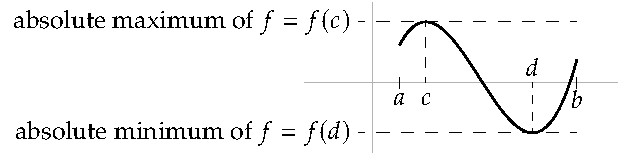
\includegraphics{../figures/minmax}
\end{center}
\end{frame}

\begin{frame}

\begin{theorem}[Min-max theorem / Extreme value theorem]
A continuous $f \colon [a,b] \to \R$ on a closed and bounded
interval $[a,b]$ 
achieves both an absolute minimum and an absolute maximum on $[a,b]$.
\end{theorem}

\pause
\textbf{Proof:}
By lemma, $f$ is bounded, so $f\bigl([a,b]\bigr)$ is bounded.

\pause
\thus~ $\exists$ seqs. $\bigl\{ f(x_n) \bigr\}_{n=1}^\infty$ and $\bigl\{ f(y_n)
\bigr\}_{n=1}^\infty$, where $x_n$ and $y_n$ are in $[a,b]$, and

$\displaystyle \lim_{n\to\infty} f(x_n) = \inf f\bigl([a,b]\bigr)$
\qquad and \qquad
$\displaystyle \lim_{n\to\infty} f(y_n) = \sup f\bigl([a,b]\bigr)$.

\pause
\medskip

$\{ x_n \}_{n=1}^\infty$ and $\{ y_n \}_{n=1}^\infty$ may not converge.

\pause
By Bolzano--Weierstrass, $\exists$
convergent subsequences
$\{ x_{n_i} \}_{i=1}^\infty$ and 
$\{ y_{m_i} \}_{i=1}^\infty$.

\pause
\medskip

Let
$\displaystyle
x \coloneqq \lim_{i\to\infty} x_{n_i}
\qquad \text{and} \qquad
y \coloneqq \lim_{i\to\infty} y_{m_i}$.

\pause
\medskip

$a \leq x_{n_i} \leq b$ for all $i$ \wthus $a \leq x \leq b$.
\pause
\qquad 
Similarly, $a \leq y \leq b$.

\pause
\medskip

$\displaystyle
\inf f\bigl([a,b]\bigr)
\pause
= \lim_{n\to\infty} f(x_n)
\pause
= \lim_{i\to\infty} f(x_{n_i})
\pause
= f \Bigl( \lim_{i\to\infty} x_{n_i} \Bigr)
\pause
= f(x)$.

\pause
$\displaystyle
\sup f\bigl([a,b]\bigr)
\pause
= \lim_{n\to\infty} f(y_n)
\pause
= \lim_{i\to\infty} f(y_{m_i})
\pause
= f \Bigl( \lim_{i\to\infty} y_{m_i} \Bigr)
\pause
= f(y)$.

\pause
\medskip

$f$ achieves an absolute minimum at $x$ and
 an absolute maximum at $y$.
\qed
\end{frame}

\begin{frame}

\textbf{Example:}
$f(x) \coloneqq x^2+1$ defined on the interval $[-1,2]$

achieves a minimum at $x=0$ when $f(0) = 1$.

\pause
$f$ achieves a maximum at $x=2$ where $f(2) = 5$.

\pause
\medskip

Domain of definition matters:

If domain is
$[-10,10]$, then the maximum of $f$ is no longer at $x=2$.

\pause
Instead the maximum would be achieved at either $x=10$ or $x=-10$.

\pause
\medskip

\textbf{Example:}
$f(x) \coloneqq x$ defined on $\R$

achieves neither a minimum, nor a maximum.

\pause
\medskip

That $[a,b]$ in the theorem is bounded is important.
\end{frame}

\begin{frame}

\textbf{Example:}
$f(x) \coloneqq \nicefrac{1}{x}$ defined on $(0,1)$

achieves neither a minimum, nor a maximum.

\pause
$f(x)$ is unbounded as $x \to 0$.

\pause
If $x \to 1$, then $f(x)$ approaches 1, but $f(x) > 1$ for any $x \in
(0,1)$.

\pause
\medskip

That $[a,b]$ in the theorem is closed is important.

\pause
\medskip

\textbf{Example:}
Define $f \colon [0,1] \to \R$ by 
$f(x) \coloneqq \nicefrac{1}{x}$ for $x > 0$ and let $f(0) \coloneqq 0$.

\pause
$f$ does not achieve a maximum.

\pause
$f$ is discontinuous at $0$.

\pause
\medskip

That $f$ is continuous in the theorem is important.
\end{frame}

\begin{frame}
\begin{lemma}
Let $f \colon [a,b] \to \R$ be continuous.
Suppose $f(a) < 0$ and $f(b) > 0$. 

\pause
Then there exists $c \in (a,b)$
such that $f(c) = 0$.
\end{lemma}

\pause
\textbf{Proof:}
Define two sequences $\{ a_n \}_{n=1}^\infty$
and $\{ b_n \}_{n=1}^\infty$ inductively:
\begin{enumerate}[(i)]
\item
\pause
Let $a_1 \coloneqq a$ and $b_1 \coloneqq b$.
\item
\pause
If $f\left(\frac{a_n+b_n}{2}\right) \geq 0$,

let $a_{n+1} \coloneqq a_n$ and
$b_{n+1} \coloneqq \frac{a_n+b_n}{2}$.
\item
\pause
If $f\left(\frac{a_n+b_n}{2}\right) < 0$,

let $a_{n+1} \coloneqq \frac{a_n+b_n}{2}$ and
$b_{n+1} \coloneqq b_n$.
\end{enumerate}

\pause
\vspace*{-1.2in}
\hspace*{2.4in}\scalebox{0.75}{
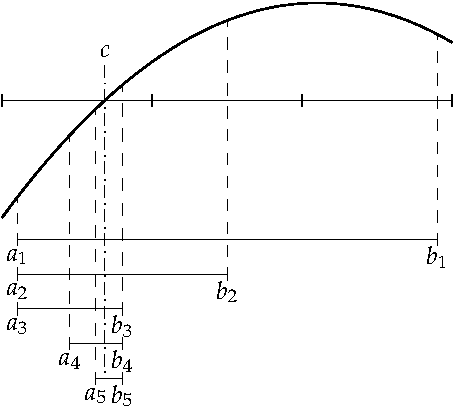
\includegraphics{../figures/bisect}
}

\pause
\vspace*{-0.8in}
If $a_n < b_n$, then $a_n < \frac{a_n+b_n}{2} < b_n$.

\pause
So $a_{n+1} < b_{n+1}$.

\pause
By induction $a_n < b_n$ for all $n$.

\pause
\medskip

Also $a_n \leq a_{n+1}$ and $b_n \geq b_{n+1}$ for all $n$.

\pause
$\{a_n\}_{n=1}^\infty$ and $\{ b_n \}_{n=1}^\infty$ are monotone.

\end{frame}

\begin{frame}
As $a_n < b_n \leq b_1 = b$ and 
$b_n > a_n \geq a_1 = a$ for all $n$,

\pause
$\{a_n\}_{n=1}^\infty$ and $\{ b_n \}_{n=1}^\infty$ are bounded.

\pause
\medskip

Thus convergent. Let ~$c \coloneqq \lim\, a_n$,~ $d \coloneqq \lim\, b_n$,
~(note $a \leq c \leq d \leq b$).

\pause
\medskip

$b_{n+1} - a_{n+1} = \frac{b_n-a_n}{2}$ for all $n$.
\pause
\qquad 
Induction \wthus
$b_n - a_n
= \frac{b_1-a_1}{2^{n-1}}
= 2^{1-n} (b-a)$.

\pause
\medskip

$\displaystyle
d-c
\pause
= \lim_{n\to\infty} (b_n - a_n)
\pause
=
\lim_{n\to\infty} 2^{1-n} (b-a)
\pause
= 0$.

\pause
\medskip

\thus \quad $d=c$.

\pause
\medskip

By construction, for all $n$, \quad
$f(a_n) < 0$ \quad and \quad $f(b_n) \geq 0$.

\pause
\medskip

As $f$ is continuous:

\medskip

$f(c)
\pause
=
f(\lim\limits_{n\to\infty} a_n)
\pause
=
\lim\limits_{n\to\infty} f(a_n)
\pause
\leq 0$
\pause
\qquad and \qquad
$f(c)
\pause
=
f(\lim\limits_{n\to\infty} b_n)
\pause
=
\lim\limits_{n\to\infty} f(b_n)
\pause
\geq 0$.

\pause
\medskip

\thus \quad $f(c) = 0$.

\pause
\medskip

Note that $c \not=a$ and $c \not= b$ as $f(c)=0$, \quad so $a < c < b$.  \qed
\end{frame}

\begin{frame}

\begin{theorem}[Bolzano's intermediate value theorem]
Let $f \colon [a,b] \to \R$ be continuous.
Suppose $y \in \R$ is such that $f(a) < y < f(b)$
or $f(a) > y > f(b)$.
\pause
Then there exists a $c \in (a,b)$
such that $f(c) = y$.
\end{theorem}

\pause
\textbf{Proof:}
If $f(a) < y < f(b)$, then define $g(x) \coloneqq f(x)-y$.

\pause

If $f(a) > y > f(b)$, then define $g(x) \coloneqq y-f(x)$.

\pause
\medskip

Then $g(a) < 0$ and $g(b) > 0$.

\pause
Apply the lemma to find $c \in (a,b)$ such that $g(c) = 0$.

\pause
\thus \quad $f(c) = y$.
\qed

\pause
\medskip

If $f \colon S \to \R$ is continuous,

we often apply the theorem to $f|_{[a,b]}$ if $[a,b] \subset S$.

\end{frame}

\begin{frame}

The proof of the lemma tells us how to find the root $c$.

\pause
\medskip

\textbf{Example:} (Bisection method)

$f(x) \coloneqq x^3-2x^2+x-1$ has a real root in $(1,2)$:

\pause
Notice that $f(1) = -1$ and $f(2) = 1$.

\pause
By Bolzano, $\exists$ $c \in (1,2)$ such that $f(c) = 0$.

\pause
\medskip

For better approximation, follow proof:

Note $f(1.5) = -0.625$, \wthus
there is a root in $(1.5,2)$.

\pause
Note $f(1.75) \approx -0.016$, \wthus
there is a root in $(1.75,2)$.

\pause
Note $f(1.875) \approx 0.44$, \wthus
there is a root in $(1.75,1.875)$.

\pause
Keep going (note that the root is approx $1.7549$)

\pause
\medskip

Bisection method works reasonably quickly (1 bit of precision per step) for any
continuous function (once you find initial interval).

\pause
\medskip

Faster techniques for nicer functions such as polynomials (e.g., Newton's).

\pause
\medskip

The theorem/technique gives one root.  Must work harder if there are more.

\end{frame}

\begin{frame}
Even degree polynomials may not have roots, e.g., 
$x^2+1$.
\pause
However,

\begin{proposition}
Let $f(x)$ be a polynomial of odd degree.  Then $f$ has a real root.
\end{proposition}

\pause
\textbf{Proof:}
Suppose ~$f(x) = a_d x^d + a_{d-1} x^{d-1} + \cdots + a_1 x + a_0$ for odd
$d$ ~($a_d \not= 0$).

\pause
Divide by $a_d$ to get a \emph{monic polynomial}:
~ $g(x) \coloneqq x^d + b_{d-1} x^{d-1} + \cdots + b_1 x + b_0$.
%($b_k = \nicefrac{a_k}{a_d}$)

\pause
\medskip

Consider $g(n)$ for $n \in \N$.

\pause
\medskip

$\displaystyle
\abs{\frac{b_{d-1} n^{d-1} + \cdots + b_1 n + b_0}{n^d}}
\pause
 =
\frac{\abs{b_{d-1} n^{d-1} + \cdots + b_1 n + b_0}}{n^d}
$

\pause
\medskip

\quad
$\displaystyle
\leq
\frac{\abs{b_{d-1}} n^{d-1} + \cdots + \abs{b_1} n + \abs{b_0}}{n^d}
\pause
\leq
\frac{\abs{b_{d-1}} n^{d-1} + \cdots + \abs{b_1} n^{d-1} + \abs{b_0} n^{d-1}}{n^d}
$

\pause
\medskip

\quad
$\displaystyle
=
\frac{n^{d-1}\bigl(\abs{b_{d-1}} + \cdots + \abs{b_1} + \abs{b_0}\bigr)}{n^d}
\pause
=
\frac{1}{n}
\bigl(\abs{b_{d-1}} + \cdots + \abs{b_1} + \abs{b_0}\bigr) .
$

\pause
\medskip

\thus \quad
$\displaystyle
\lim_{n\to\infty} \frac{b_{d-1} n^{d-1} + \cdots + b_1 n + b_0}{n^d}
= 0$.

\end{frame}

\begin{frame}

\thus \quad $\exists$ $M \in \N$ \quad such that 
\quad
$\displaystyle \abs{\frac{b_{d-1} M^{d-1} + \cdots + b_1 M + b_0}{M^d}} < 1$.

\pause
\medskip

\thus \quad 
$\displaystyle
-(b_{d-1} M^{d-1} + \cdots + b_1 M + b_0) < M^d$
\pause
\wthus
$g(M) > 0$.

\pause
\medskip

An exercise (similar as above):
$\exists$ $K \in \N$ such that
$b_{d-1} {(-K)}^{d-1} + \cdots + b_1 (-K) + b_0 < K^d$
\wthus $g(-K) < 0$

\pause
\medskip

Hint: Make sure you use that $d$ is odd: If $d$ is odd, then ${(-n)}^d = -(n^d)$.

\pause
\medskip

Intermediate value theorem implies $\exists$
$c \in (-K,M)$, such that $g(c) = 0$.

\pause
\medskip

As $g(x) = \frac{f(x)}{a_d}$, then $f(c) = 0$.
\qed
\end{frame}

\begin{frame}

\textbf{Example:}
There exist discontinuous functions with
the intermediate value property.
\pause
E.g.,
\begin{equation*}
f(x) \coloneqq
\begin{cases}
\sin(\nicefrac{1}{x}) & \text{if } x \not= 0, \\
0 & \text{if } x=0,
\end{cases}
\end{equation*}
is not continuous at $0$; however, $f$ has the intermediate value property:

\pause
\medskip

If $a < b$ and $y$ is such that $f(a) < y < f(b)$ or $f(a) > y > f(b)$,

then $\exists$ $c \in (a,b)$ such that $f(c) = y$.

\pause
\medskip

Proof is an exercise.
\end{frame}

\begin{frame}

Combining theorems of this section:

\begin{corollary}
If $f \colon [a,b] \to \R$ is continuous, then the direct image
$f\bigl([a,b]\bigr)$
is a closed and bounded interval or a single number.
\end{corollary}

\pause
\begin{center}
\subimport*{../figures/}{figimageinterval.pdf_t}
\end{center}

\pause
\textbf{Proof:} Exercise.

\end{frame}

\end{document}
